%%%---PREAMBLE---%%%%%%%%%%%%%%%%%%%%%%%%%%%%
\documentclass[oneside,12pt,final]{ucthesis-CA2012}
% \documentclass[oneside,12pt,final]{ucthesis}
\pdfoutput=1

% jpp note: see:
%
% http://www.graddiv.ucsb.edu/docs/default-source/default-document-library/guide-to-formatting-filing-theses-dissertations.pdf?sfvrsn=0
%
% University of California, Santa Barbara
% Guide to Formatting and Filing Theses, Dissertations, and DMA Supporting Documents
% 2016-17

%--- Packages ---------------------------------------------------------
\usepackage[lofdepth,lotdepth,caption=false]{subfig}
\usepackage{fancyhdr}
\usepackage{hyperref}
\usepackage{amsmath, amssymb, graphicx} 
\usepackage{xspace}
\usepackage{braket}
\usepackage{color}
\usepackage{setspace}
% \usepackage{subfigure} (Subfigure package clashes with another package)
% \usepackage{subfig}
\usepackage{bm,ushort} % Needed for UAV coordination chapter




%%%%%%%%%%%%%%%%%%%%%%%%%
% Pandoc

\usepackage{fancyvrb}
\newcommand{\VerbBar}{|}
\newcommand{\VERB}{\Verb[commandchars=\\\{\}]}
\DefineVerbatimEnvironment{Highlighting}{Verbatim}{commandchars=\\\{\}}
% Add ',fontsize=\small' for more characters per line
\newenvironment{Shaded}{}{}
\newcommand{\KeywordTok}[1]{\textcolor[rgb]{0.00,0.44,0.13}{\textbf{#1}}}
\newcommand{\DataTypeTok}[1]{\textcolor[rgb]{0.56,0.13,0.00}{#1}}
\newcommand{\DecValTok}[1]{\textcolor[rgb]{0.25,0.63,0.44}{#1}}
\newcommand{\BaseNTok}[1]{\textcolor[rgb]{0.25,0.63,0.44}{#1}}
\newcommand{\FloatTok}[1]{\textcolor[rgb]{0.25,0.63,0.44}{#1}}
\newcommand{\ConstantTok}[1]{\textcolor[rgb]{0.53,0.00,0.00}{#1}}
\newcommand{\CharTok}[1]{\textcolor[rgb]{0.25,0.44,0.63}{#1}}
\newcommand{\SpecialCharTok}[1]{\textcolor[rgb]{0.25,0.44,0.63}{#1}}
\newcommand{\StringTok}[1]{\textcolor[rgb]{0.25,0.44,0.63}{#1}}
\newcommand{\VerbatimStringTok}[1]{\textcolor[rgb]{0.25,0.44,0.63}{#1}}
\newcommand{\SpecialStringTok}[1]{\textcolor[rgb]{0.73,0.40,0.53}{#1}}
\newcommand{\ImportTok}[1]{#1}
\newcommand{\CommentTok}[1]{\textcolor[rgb]{0.38,0.63,0.69}{\textit{#1}}}
\newcommand{\DocumentationTok}[1]{\textcolor[rgb]{0.73,0.13,0.13}{\textit{#1}}}
\newcommand{\AnnotationTok}[1]{\textcolor[rgb]{0.38,0.63,0.69}{\textbf{\textit{#1}}}}
\newcommand{\CommentVarTok}[1]{\textcolor[rgb]{0.38,0.63,0.69}{\textbf{\textit{#1}}}}
\newcommand{\OtherTok}[1]{\textcolor[rgb]{0.00,0.44,0.13}{#1}}
\newcommand{\FunctionTok}[1]{\textcolor[rgb]{0.02,0.16,0.49}{#1}}
\newcommand{\VariableTok}[1]{\textcolor[rgb]{0.10,0.09,0.49}{#1}}
\newcommand{\ControlFlowTok}[1]{\textcolor[rgb]{0.00,0.44,0.13}{\textbf{#1}}}
\newcommand{\OperatorTok}[1]{\textcolor[rgb]{0.40,0.40,0.40}{#1}}
\newcommand{\BuiltInTok}[1]{#1}
\newcommand{\ExtensionTok}[1]{#1}
\newcommand{\PreprocessorTok}[1]{\textcolor[rgb]{0.74,0.48,0.00}{#1}}
\newcommand{\AttributeTok}[1]{\textcolor[rgb]{0.49,0.56,0.16}{#1}}
\newcommand{\RegionMarkerTok}[1]{#1}
\newcommand{\InformationTok}[1]{\textcolor[rgb]{0.38,0.63,0.69}{\textbf{\textit{#1}}}}
\newcommand{\WarningTok}[1]{\textcolor[rgb]{0.38,0.63,0.69}{\textbf{\textit{#1}}}}
\newcommand{\AlertTok}[1]{\textcolor[rgb]{1.00,0.00,0.00}{\textbf{#1}}}
\newcommand{\ErrorTok}[1]{\textcolor[rgb]{1.00,0.00,0.00}{\textbf{#1}}}
\newcommand{\NormalTok}[1]{#1}
\usepackage{graphicx,grffile}


\providecommand{\tightlist}{%
  \setlength{\itemsep}{0pt}\setlength{\parskip}{0pt}}



%%%%%%%%%%%%%%%%%%%%%%%%%
% end pandoc
%%%%%%%%%%%%%%%%%%%%%%%%%

















%---New Definitions and Commands------------------------------------------------------
\def\p{\partial}
\def\im{\mrm{im}}
\def\Tr{\mrm{Tr}}
%\def\Z{\mbb{Z}}
%\def\R{\mbb{R}}
%\def\C{\mbb{C}}
\def\half{\frac{1}{2}}
\def\filler{\phantom{fillerfillerfiller}}
\newcommand{\be}{\begin{equation}}
\newcommand{\ee}{\end{equation}}
\newcommand{\mbb}[1]{\mathbb{#1}}
\newcommand{\mrm}[1]{\mathrm{#1}}
\newcommand{\mcal}[1]{\mathcal{#1}}
\newcommand{\mbf}[1]{\mathbf{#1}}
\newcommand{\ph}[1]{\phantom{#1}}
\newcommand{\udten}[3]{#1^{#2}_{\ph{#2}#3}}
\newcommand{\duten}[3]{#1^{\ph{#2}#3}_{#2}}
\newcommand{\pd}[2]{\frac{\p#1}{\p#2}}
\newcommand{\D}[2]{\frac{d#1}{d#2}}

% %%% Needed for UAV coordination chapter
% \newcommand{\frk}{\mathfrak}               
% \newcommand{\cl}{\mathcal}
% %%%

%---Set Margins ------------------------------------------------------

% jpp note: for double-spacing:
% \def\dsp{\def\baselinestretch{1}\large\normalsize} % jpp
\def\dsp{\def\baselinestretch{2}\large\normalsize} % jpp
% originally defined in 
% in ucthesis-CA2012.cls

\setlength\oddsidemargin{0.25 in} 
\setlength\evensidemargin{0.25 in} 
\setlength\textwidth{6.25 in} 
\setlength\textheight{8.50 in}
\setlength\footskip{0.25 in} 
\setlength\topmargin{0 in} 
\setlength\headheight{0.25 in} 
\setlength\headsep{0.25 in}


% % jpp customizations (generous margins)
\setlength\textwidth{5.7 in} 
\setlength\textheight{8.4 in}
\setlength\footskip{0.45 in} 
\setlength\topmargin{0 in} 
\setlength\evensidemargin{0.5 in} 
\setlength\oddsidemargin{0.5 in} 


% jpp customizations (thin margins for draft printing)
% \usepackage[letterpaper, margin=.2in]{geometry}



%%%%%%%%%%%%%%%%%%%%%%%%%%%%%%%%%%%%%%%%%%%%%%%%%%%%
%%%%%%%%%%%%%%%     David's Additions    %%%%%%%%%%%%%%%%%%%%%%%%%%
%%%%%%%%%%%%%%%%%%%%%%%%%%%%%%%%%%%%%%%%%%%%%%%%%%%%

% \usepackage{amsmath,amssymb,amsfonts}
%\usepackage{url}
%\usepackage{fullpage}
% \usepackage{setspace}      % \singlespace, \doublespace \onehalfspacing
% \usepackage{ifthen}      % \ifthenelse,\boolean,\newboolean,\setboolean
% \usepackage{mathptmx} % slightly more compressed font.
%\usepackage[T1]{fontenc}\usepackage[condensed,math]{kurier} % fancy font
% \usepackage{makeidx}  % to make a keyword index: \index{}
% \usepackage{showidx}  % prints index entries in the left margin (debug)
% \usepackage{needspace}     % \needspace{5\baselineskip} no page breaks for 5 lines
% \usepackage{mparhack} % correct Latex bug in \marginpar
% \usepackage{chemarr}  % arrows 4 chem: \xrightleftharpoons[]{} \xrightarrow{}
\usepackage{listings} % source code printer for latex
\lstset{language=Matlab}
\lstset{basicstyle=\small,morekeywords={cvx_begin,cvx_end,variables,maximize,minimize,subject,to,linprog,quadprog,ones,optimset}}

%%%% Figure packages
%\usepackage{graphicx}
 \usepackage{pstool}           % \psfrag for pdflatex -- preferable(?), not transparent
% \usepackage{auto-pst-pdf}      % \psfrag & PStricks for pdflatex -- transparent!!!
% \usepackage[pdftex]{graphics}
%\usepackage{subfigure}         % \subfigure[a]{\includegraphics\ldots\label{fi:\ldots}}
% \usepackage{sidecaption}       % \sidecaption (to be placed inside figure env.
% \graphicspath{{./figuresdir1/}{./figuresdir2/}{./figuresdir3/}}
% \graphicspath{{./figures}} % david
\graphicspath{{./figures}} % not sure why double {{ necessary. See
                           % http://en.wikibooks.org/wiki/LaTeX/Importing_Graphics 
\DeclareGraphicsExtensions{.pdf,.jpg,.eps,.png}


%%%%%%%%%%%%%%%%%%%%%%%%%%

%%%% Bibliography packages (order is important)
% \usepackage{bibentry}% \nobibliography* \ldots  \bibentry{..} inserts a bib entry
% apparently incompatible with hyperef
% \makeatletter\let\NAT@parse\undefined\makeatother % enbl natbib with IEEE cls
%\usepackage[numbers,sort&compress,sectionbib]{natbib} % \cite,\citet,\citep,\ldots
%\usepackage[letterpaper,colorlinks=true,linkcolor=blue,backref=page]{hyperref}
%\renewcommand*{\backref}[1]{\small (cited in p.~#1)}
%\usepackage[norefs,nocites]{refcheck} % options:norefs,nocites,msgs,chkunlbld
%%%%%%%%%%%%%%%%%%%%%%%%%%

\usepackage[draft,fancythm,fancybb,morse]{jphmacros2e}
% \usepackage[elsart,draft,fancythm,fancybb,morse]{jphmacros2e}


% \usepackage{algorithm2e} % algorithms, see https://www.sharelatex.com/learn/Algorithms
% arg, joao defined algorithm environment already. Use this instead:
\usepackage{algorithmic}
% Seems to be preferred for IEEE journals according to
% https://en.wikibooks.org/wiki/LaTeX/Algorithms#Typesetting_using_the_algorithmic_package
% NOTE: I think this has to go after usepackage{jphmacros} because
% joao defines the algorithm environment for something else, and I
% want to write over his def'n. 


% Overruns margin: \section{Sufficient condition for stability with limited-communication encoders}
% https://tex.stackexchange.com/questions/195885/margins-of-section-title-is-out-of-bounds
\usepackage{blindtext}
\usepackage[raggedright]{titlesec}


%% Macros & options for this Document

%\DeclareMathOperator{\id}{id}

\allowdisplaybreaks

% \makeindex

\newcommand{\david}[1]{\drafttext{\footnote{\drafttext{David: #1}}}}
%\renewcommand{\l}{\operatorname{\ell}}     % l space



%%%%%%%%%%%%%%%%%%%%%%%%%%%%%%%%%%%%%%%%%%%%%%%%%%%%
%%%%%%%%%%%%%%%    End David's Additions    %%%%%%%%%%%%%%%%%%%%%%%
%%%%%%%%%%%%%%%%%%%%%%%%%%%%%%%%%%%%%%%%%%%%%%%%%%%%




\newlength{\figwidth}
\setlength{\figwidth}{.9\textwidth}







%%%%%%%%%%%%%%%%%%%%%%%%%%%%%%%%%%%%%%%%%%%%%%%%
%% Justin's terminology

% We've had many names for the following concept: Given an encoder,
% max over all possible symbol streams that the encoder may emit, the
% average number of non-free symbols in that symbol stream. We denote
% this $\gamma_{\max}$, but we've used:
% 0. Average fraction of non-free symbols
% 1. Average energy
% 2. Average power
% 3. Average communication
% 4. Average cost-per-symbol
% ... so let's have a macro for it:
\newcommand{\avecost}{average cost per symbol}

% We've changed the definition of 'bit-rate' a couple times, so
% 'average bit-rate' may not be as appropriate as just 'bit-rate' now.
% 2014-09-22: We changed it back, 'average' is now appropriate. :)
\newcommand{\bitrate}{average bit-rate}
\newcommand{\bitrates}{average bit-rates}
\newcommand{\abitrate}{an average bit-rate}

% We've had differing opinions about using "seconds" or "time units". 
\newcommand{\timeunit}{time unit}
\newcommand{\timeunits}{time units}

% We've had differing opinions about "process (1)" vs "the process (1)".
% 2016-03-26: reviewer says use "process (1)" for everything. Fine.
\newcommand{\theprocess}{process \eqref{eq:full-process}}
\newcommand{\thescalarprocess}{process \eqref{eq:scalar-process}}
\newcommand{\process}{process \eqref{eq:full-process}}
\newcommand{\theunstableprocess}{process \eqref{eq:process-unstable-subspace}}

% Let's be consistent with our "sum of unstable eigenvalues"
% expression.
% Note: 2015-06-29 we decided to use strict ineq in the sum of
% eigs. I'll just hack it and change sumeigs too.

\newcommand{\sumeigs}{ \sum_{i:\Re\lambda_i[A] > 0}\lambda_i[A] }
\newcommand{\sumeigsstrict}{ \sum_{i:\Re\lambda_i[A] > 0}\lambda_i[A] }
\newcommand{\sumeigsplus}{ \sum_{i:\Re\lambda_i[A_+] \ge 0}\lambda_i[A_+] }

% How to refer to each of the n scalar encoder/decoder pairs that we use in proof of Lem 4 and event-based?
\newcommand{\subenc}{sub-encoder}
\newcommand{\subencs}{sub-encoders}
\newcommand{\Subenc}{Sub-encoder}
\newcommand{\subdec}{sub-decoder}
\newcommand{\Subdec}{Sub-decoder}
\newcommand{\subdecs}{sub-decoders}

% We've vascillated over time about whether to refer to the maximum
% allowable average power (average cost) as \gamma_{\max} or just
% \gamma.
% \newcommand{\gmax}{\gamma_{\max}}
\newcommand{\gmax}{\gamma}

\newcommand{\tauu}{\underline{\tau}}

\newcommand{\nonfree}{non-free}


% Adds padding around table entries. (Q: What table?)
% http://tex.stackexchange.com/questions/64761/add-just-a-little-more-padding-to-my-table
% \renewcommand{\arraystretch}{2}  

% In 'there exists x such that...', is 'such that' a pipe or colon?
\newcommand{\suchthat}{:}

% Least-common multiple time period 
\newcommand{\Tlcm}{T_0}

% Event-based mag and angle encoder time periods
% \newcommand{\Tr}{T_\rho}
\newcommand{\Tth}{T_\theta}

% The string of symbols produced by the encoder from t=0 to t=t,
% starting from IC x_0: \encoder(t)
\DeclareMathOperator{\encoder}{\mathbf{Enc}}

% The overline notation for "the midpoint of an interval" is maybe
% confusing, so let's try this:
\DeclareMathOperator{\midpoint}{\mathbf{mid}}


% From http://www.math.rochester.edu/mathfolk/help/tex-style-files/thesis/urcsmacros.tex
%
% various latin abbreviations
%
\def\adhoc{{\em ad hoc}}
\def\aposteriori{{\em a posteriori}}
\def\apriori{{\em a priori}}
\def\Cf{{\em Cf.}}
\def\cf{{\em cf.}}
\def\Eg{{\em E.g.}}
\def\eg{{\em e.g.}}
\def\etal{{\em et al.}}
\def\etc{{\em etc.}}
\def\Ibid{{\em Ibid.}}
\def\ibid{{\em ibid.}}
\def\Id{{\em Id.}}
\def\id{{\em id.}}
\def\Ie{{\em I.e.}}
\def\ie{{\em i.e.}}


% differentiating 1-d and 2-d error vectors
\usepackage{bm}  % bold math
\def\ee{{\bm{e}}}




%%%%%%%%%%%%%%%%%%%%%%%%%%%%%%%%%%%%%%%%%%%%%%%%%%%
% Justin's random preamble stuff from MINENG

%% From Daniel Lieberzon:
% \usepackage{cancel} % \cancel{}, \bcancel{}, \xcancel{}, \cancelto{}{}

\DeclareMathOperator{\prob}{\mathbb{P}}
\DeclareMathOperator{\diam}{{\textbf{diam}}}
  
\renewcommand{\PReal}{{\Real_{>0}}}          % Set of Positive Real Numbers
\renewcommand{\NNReal}{{\Real_{\ge 0}}}         % Set of Non Negative Real Numbers

% Daniel: Get rid of the \qed signs at the end of statements to save
% space. They are only needed at the end of proofs.
\renewcommand{\frqed}{}


%%
% for longer draft notes which won't fit in the footnotes. (JPP, 2012.05.23)
\newcommand{\draftnoteinline}[1]{
\vspace{5mm}
{\footnotesize 
$\ddot\smile$ {\bf #1 } $\ddot\smile$}
\vspace{5mm}
} 

\newcommand{\notetoself}[1]{
\rule{\textwidth}{1pt} %

\vspace{5mm} %
{\footnotesize  %
$\ddot\smile$ { #1 } $\ddot\smile$} %
\vspace{5mm} %

\rule{\textwidth}{1pt} %
} 


\newcommand{\notetoselfhide}[1]{}


\providecommand{\joao}[1]{\footnote{\drafttext{Joao: #1}}}
\newcommand{\justin}[1]{\footnote{\drafttext{Justin: #1}}}

% END justin's preamble stuff
%%%%%%%%%%%%%%%%%%%%%%%%%%%%%%%%%%%%%%%%%%


%%%%%%%%%%%%%%%%%%%%
% START Justin from cyclops paper



\renewcommand{\r}{\textcolor{red}}
\renewcommand{\b}{\textcolor{blue}}
\newcommand{\cmark}{\ding{51}}%
\newcommand{\xmark}{\ding{55}}%

% \DeclarePairedDelimiter\ceil{\lceil}{\rceil}
% \DeclarePairedDelimiter\floor{\lfloor}{\rfloor}
% \DeclareMathOperator*{\argmin}{\arg\!\min}
% \DeclareMathOperator*{\argmax}{\arg\!\max}
% \DeclarePairedDelimiter{\abs}{\lvert}{\rvert}
% \DeclarePairedDelimiter{\norm}{\lVert}{\rVert}
%\usepackage{achemso}
%s\setlength{\bibsep}{0pt}
%\usepackage{titling}

%%%%%%%%%%%%%%%%%%
\newcommand{\eco}{\text{$\mathbb{EN}$}}
%\newcommand{\encFHE}[2]{\text{ENC}^{\text{FHE}}_{#1}(#2)}
%\newcommand{\encPHE}[2]{\text{ENC}^{\text{PHE}}_{#1}(#2)}

%\newcommand{\decFHE}[2]{\text{DEC}^{\text{FHE}}_{#1}(#2)}
%\newcommand{\decPHE}[2]{\text{DEC}^{\text{PHE}}_{#1}(#2)}


%\newcommand{\encPHE}[2]{\llbracket #2 \rrbracket_{#1}}
%\newcommand{\decPHE}[2]{\texttt{DEC}^{\text{PHE}}_{#1}(#2)}
\newcommand{\encPHE}[1]{\llbracket #1\rrbracket}
\newcommand{\decPHE}{\texttt{DEC}}

\renewcommand{\Re}{{\mathbb{R}}}
% \newcommand{\R}{{\mathbb{R}}}
\newcommand{\Ze}{{\mathbb Z}}
%\newcommand{\sys}{\textbf{SelCon }} 
\newcommand{\sys}{SeleCon } 

% correct bad hyphenation here
\hyphenation{op-tical net-works semi-conduc-tor limit-ed-comm-uni-cat-ion}


% maybe should go after begin{document}?

\definecolor{codegreen}{rgb}{0,0.6,0}
\definecolor{codegray}{rgb}{0.5,0.5,0.5}
\definecolor{codepurple}{rgb}{0,0,0.82}
\definecolor{backcolour}{rgb}{1,1,1}
 
\lstdefinestyle{mystyle}{
    backgroundcolor=\color{backcolour},   
    commentstyle=\color{codegreen},
    keywordstyle=\scriptsize\color{blue},
    numberstyle=\tiny\color{codegray},
    stringstyle=\scriptsize\color{codepurple},
    basicstyle=\scriptsize,
    %frame=single,
    breakatwhitespace=false,         
    breaklines=true,                 
    captionpos=t,                    
    keepspaces=true,                             
    showspaces=false,                
    showstringspaces=false,
    showtabs=false,                  
    tabsize=2,
    belowcaptionskip=0.5em,
    aboveskip=0.3em,
    belowskip=0.3em,
    moredelim=**[is][\color{blue}]{@}{@},
    emph={%  
    assert_pin, WAIT_US, deassert_pin%
    },emphstyle={\color{red}}%
}

\lstset{style=mystyle}
% end maybe


% END Justin from cyclops
%%%%%%%%%%%%%%%%%%%%%%%%%%


%%%%%%%%%%%%%%%%%%%%%%%%%%%%%%%%%%%%%%%%%
% BEGIN Justin from CDC 2017 rejected paper



% \DeclareMathOperator{\id}{id}



% We've had differing opinions about using ``seconds'' or ``time units''. 
% \newcommand{\timeunit}{time unit}
% \newcommand{\timeunits}{time units}

% Not sure if we should call it a ``real-time unit'' or a ``real-time processor''.
% Just use \rtu\ and change this def later.
\newcommand{\rtu}{real-time unit}
\newcommand{\Rtu}{Real-time unit}
\newcommand{\RTU}{RTU}

% Same with ``real-time I/O coprocessor''.
\newcommand{\rtio}{real-time I/O coprocessor}

\newcommand{\uC}{microcontroller}
\newcommand{\uCs}{microcontrollers}

\newcommand{\timestamp}{time-stamp}
\newcommand{\timestamps}{time-stamps}
\newcommand{\timestamped}{time-stamped}

\hyphenation{time-stamp}
\hyphenation{time-stamps}
\hyphenation{time-stamp-ed}
\hyphenation{time-stamp-ing}
\hyphenation{Free-RTOS}

% END Justin from CDC 2017


% justin hacks to expand spacing & margins, see Jason & Josh's theses

% \usepackage{setspace}
% \setlength{\parindent}{4em}
% \setlength{\parskip}{1em}
% \renewcommand{\baselinestretch}{2.5}
 % \setlength{\baselineskip}{2em}
 % \linespread{2}



\usepackage{lipsum}

% https://tex.stackexchange.com/questions/66896/ref-chapter-name-in-latex
\usepackage{nameref}



%%%---DOCUMENT---%%%%%%%%%%%%%%%%%%%%%%%%%%%%
\begin{document}

%=== Preliminary Pages ============================================
\begin{frontmatter}

    \title{Control under energy and time constraints}

    \author{Justin Payne Pearson}

    \report{Dissertation} 
    \Degree{Doctor of Philosophy} 
    \degreemonth{March} 
    \degreeyear{2018}
    \defensemonth{January}
    \defenseyear{2018}

    \chair{Professor Jo\~ao P. Hespanha} 
    \othermemberA{Professor Andrew R. Teel} 
    \othermemberB{Professor Jason R. Marden}   
    \othermemberC{Professor Amr El Abbadi}
    \numberofmembers{4}

    \field{Electrical and Computer Engineering}
    \campus{Santa Barbara}

    \maketitle
    \approvalpage
    \copyrightpage

    \begin{dedication}
        \bigskip

${}$ \\

\bigskip

${}$ \\

\bigskip

${}$ \\

\bigskip

\begin{center}
\begin{Large}
To Jen.

\bigskip

Note: Joao gave me the following advice: 

\bigskip

"Regarding the thesis, my main suggestion if to write a nice introduction that talks about state of the art and summarizes the key results. This allows the reader to easily pick and choose the chapter that he/she may find more interesting to explore further."

\end{Large}
\end{center}
    \end{dedication} 

% \dsp
% \def\baselinestretch{2}\large\normalsize

    \begin{acknowledgements}
        \addcontentsline{toc}{chapter}{Acknowledgements}
        { \setlength{\parindent}{0cm}

I'm very thankful to have met so many nice people during my graduate school career at UC Santa Barbara. 

{\bf Jo\~ao Hespanha}

Jo\~ao is the best

{\bf Andy Teel}

Andy is so cool

{\bf Jason Marden}

Jason is a neat guy

{\bf Amr El Abbadi}

Professor El Abbadi is awesome

{\bf Funding Agencies}

{\bf CCDC }

{\bf Colleagues}

{\bf Teachers}

{\bf Staff}

{\bf Family and Friends}

} % noindent
    \end{acknowledgements} 

    \begin{vitae}
        \addcontentsline{toc}{chapter}{Curriculum Vitae}
        
\begin{vitaesection}{Education}
\vspace{-0.1cm}
\item [2018]    Ph.D. in Electrical and Computer Engineering (Expected), University of California, Santa Barbara
\item [2007]    M.S. in Mechanical Engineering, Stanford University
\item [2006]    B.S. in Mechanical Engineering, University of California, Santa Barbara
\end{vitaesection}

\begin{vitaesection}{Experience}
\vspace{-0.1cm}
\item [2012 -- 2017] Graduate Student Researcher, University of California, Santa Barbara
\item [2008 -- 2012] Controls Engineer, AeroVironment
\item [2016] Instructor of Record, {\it COMP 150: Introduction to Object Oriented Programming}, California State University at Channel Islands
\item [2015] Certificate in College and University Teaching, UCSB
\item [2015] Mentor, Robotics internship, Institute for Collaborative Biotechnology, UCSB
\item [2015] Instructor of Record, {\it ENGR 3: Introduction to Programming}, UCSB
\item [2015] Mentor, School of Scientific Thought, Center for Science and Engineering Partnerships, UCSB
\item [2014] Teaching Assistant, {\it ENGR 3: Introduction to Programming}, UCSB
\item [2014] Teaching Assistant, {\it ECE 147C: Control System Design Project}, UCSB
\end{vitaesection}


\textbf{Publications}

\vspace{-0.1cm}


\vspace{0.1cm}

A. Alanwar, F. M. Anwar, Y. Zhang, J. Pearson, J. Hespanha, M. B. Srivastava. ``Cyclops: PRU Programming Framework for Precise Timing Applications.'' {\it Proc. of the 2017 IEEE International Symposium on Precision Clock Synchronization for Measurement, Control, and Communication (ISPCS)}, Aug. 2017. 

\vspace{0.1cm}

J. Pearson, J. Hespanha, D. Liberzon. ``Control with minimal cost-per-symbol encoding and quasi-optimality of event-based encoders.'' {\it IEEE Transactions on Automatic Control}, May 2017. 

\vspace{0.1cm}

J. Pearson, J. Hespanha, D. Liberzon. ``Quasi-optimality of event-based encoders.'' {\it Proc. of the 54th Conference on Decision and Control}, Dec. 2015.

\vspace{0.1cm}

J. Pearson, J. Hespanha, D. Liberzon. ``Control with Minimum Communication Cost per Symbol.'' {\it Proc. of the 53nd Conference on Decision and Control}, Dec. 2014.

    \end{vitae}

    \begin{abstract}
        \addcontentsline{toc}{chapter}{Abstract}
        % %max 350 words

The performance of a control system is often limited by constraints on timing, bandwidth, and energy. This dissertation explores the trade-offs between constraints on these resources, the control system performance, and the system to be controlled.

In this work we solve every problem ever.
        %\abstractsignature
    \end{abstract}

    \tableofcontents
    \listoffigures
    \listoftables

\end{frontmatter}





\begin{mainmatter}

    %%%%%%%%%%%%%%%%%%%%%%%%%%%%%%%%
    % Dumb crap from Grad Div 

    %---Set Headers and Footers ------------------------------------------------------
    \pagestyle{fancy}
    \renewcommand{\chaptermark}[1]{\markboth{{\sf #1 \hspace*{\fill} Chapter~\thechapter}}{} }
    \renewcommand{\sectionmark}[1]{\markright{ {\sf Section~\thesection \hspace*{\fill} #1 }}}
    \fancyhf{}

    \makeatletter \if@twoside \fancyhead[LO]{\small \rightmark} \fancyhead[RE]{\small\leftmark} \else \fancyhead[LO]{\small\leftmark}
    \fancyhead[RE]{\small\rightmark} \fi

    \def\cleardoublepage{\clearpage\if@openright \ifodd\c@page\else
      \hbox{}
      \vspace*{\fill}
      \begin{center}
        This page intentionally left blank
      \end{center}
      \vspace{\fill}
      \thispagestyle{plain}
      \newpage
      \fi \fi}
    \makeatother
    \fancyfoot[c]{\textrm{\textup{\thepage}}} % page number
    \fancyfoot[C]{\thepage}
    % \renewcommand{\headrulewidth}{0.4pt}

    \fancypagestyle{plain} { \fancyhf{} \fancyfoot[C]{\thepage}
    % \renewcommand{\headrulewidth}{10pt}
    % \renewcommand{\footrulewidth}{0pt}
    }


    % END: Dumb crap from Grad Div 
    %%%%%%%%%%%%%%%%%%%%%%%%%%%%%%%%%




% \onehalfspacing % from spacings 
% \singlespacing
% \renewcommand{\baselinestretch}{2.5}
% \linespread{2}
% \def\baselinestretch{2}\large\normalsize

% \part{Theory}
% \chapter{MinEng}
% % \lipsum[1-10]
% \part{Timing on BBB}
% \chapter{The BBB}


    %!TEX root = ../Pearson_UCSB_thesis.tex

\chapter{Introduction}
\label{chap:intro}


Control systems are frequently hampered by constraints on resources like limits on bandwidth, energy, and processor speed. 

This work explores the theoretical and practical trade-offs between these resources and control system performance. It consists of three chapters, each summarized next.



% %=========================================================
\section*{\nameref{chap:mineng} (Chapter~\ref{chap:mineng})}
% %=========================================================

Chapter~\ref{chap:mineng} considers the problem of stabilizing a continuous-time linear
time-invariant process subject to communication constraints. The basic setup is shown in Figure~\ref{fig:block_diagram2}, 
in which a finite capacity communication channel connects the
process sensors to the controller/actuator. An encoder at the sensor
sends a symbol through the channel once per sampling time, and the
controller determines the actuation signal based on the incoming
stream of symbols. The question arises: what is the smallest channel
\bitrate{} for which a given process can be stabilized? 

\begin{figure}[h]
  \psfrag{texu}{$u$}
  \centering
%  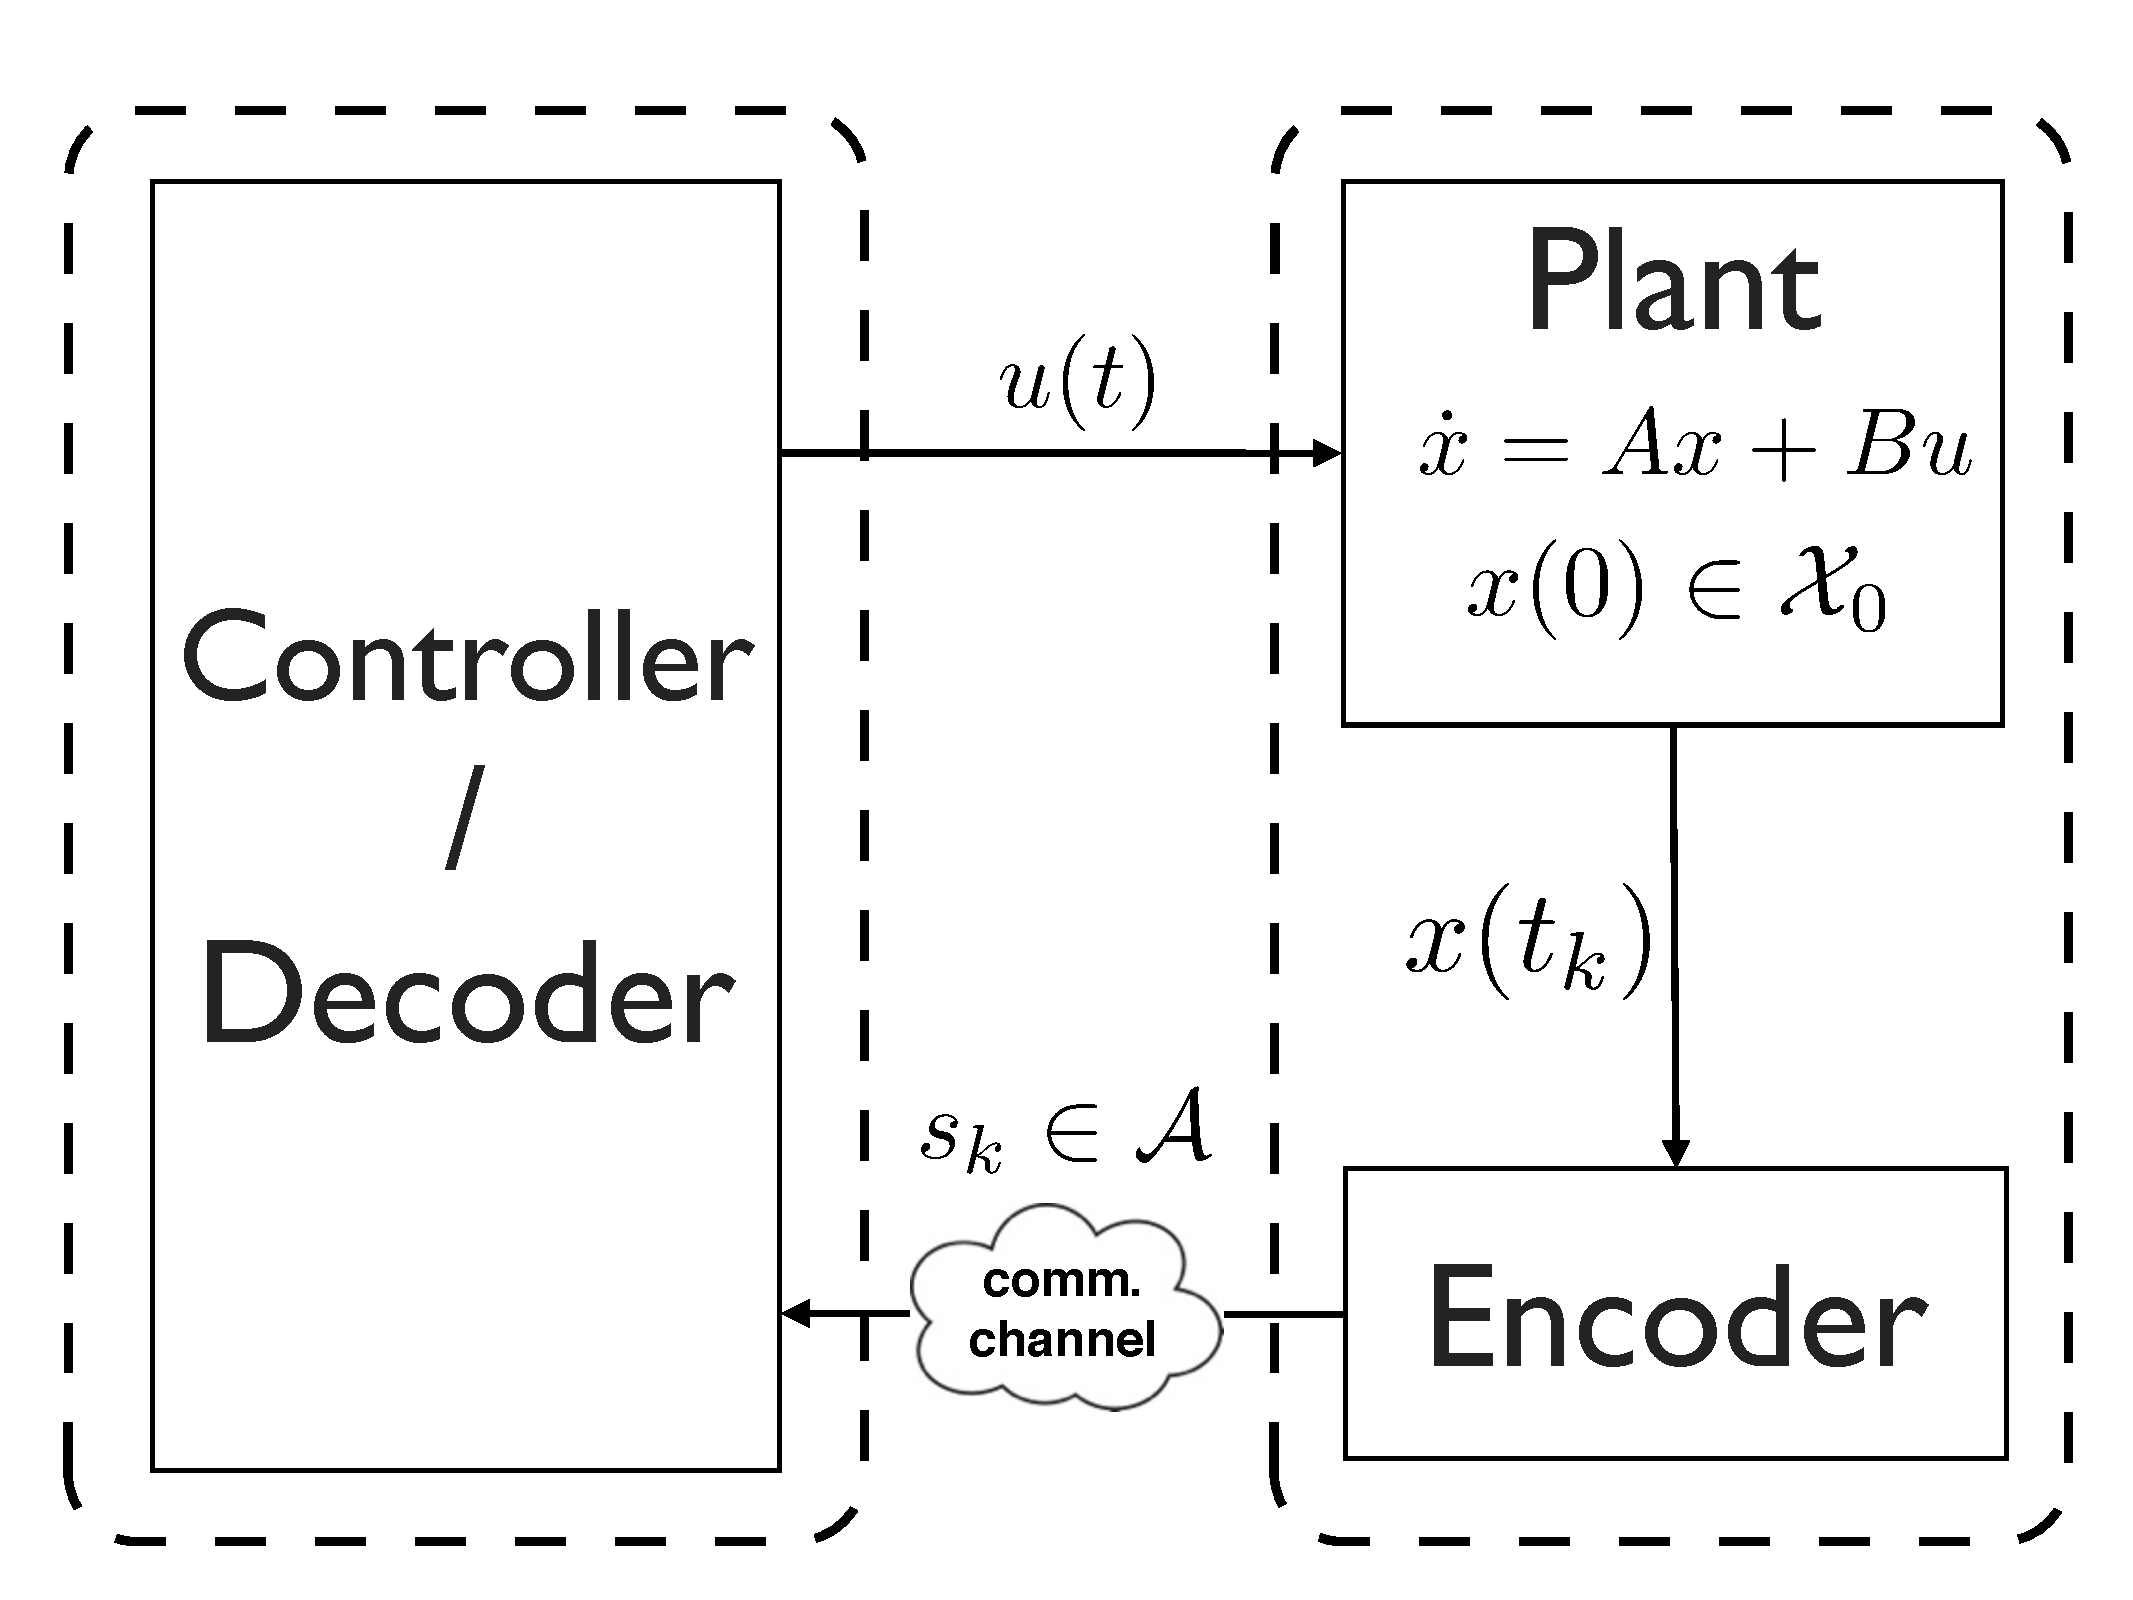
\includegraphics[angle=0,totalheight=.25\textheight]{figures/block-diagram}
  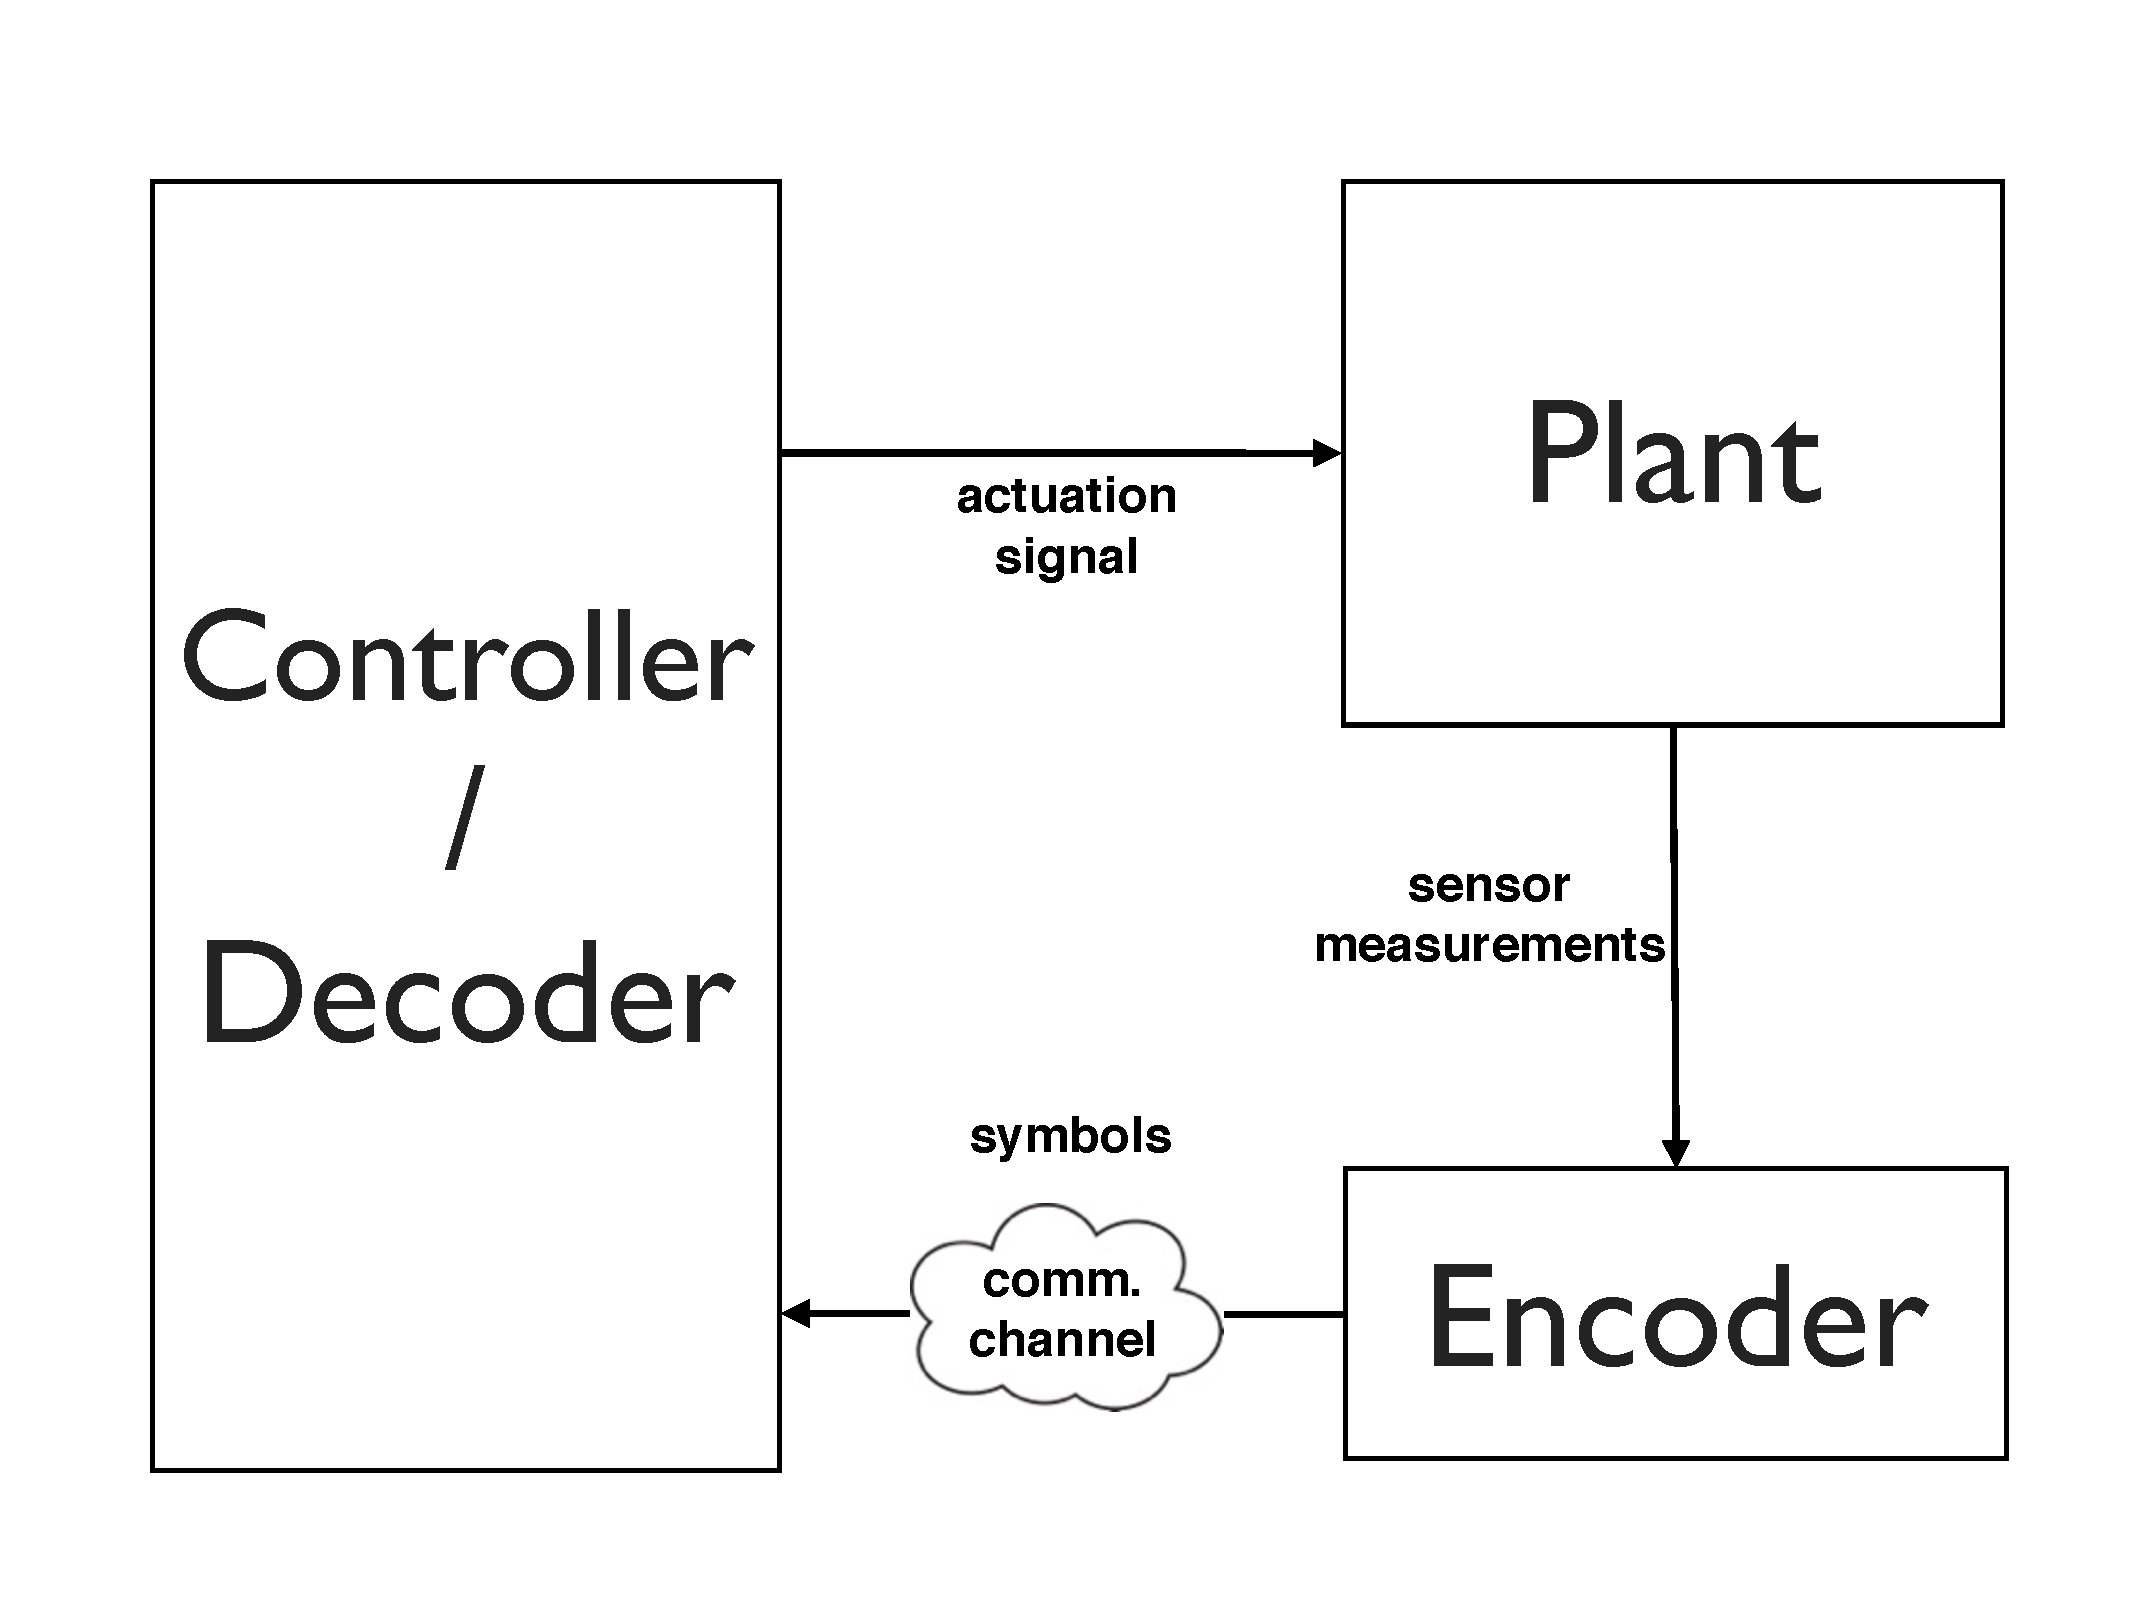
\includegraphics[angle=0,width=\figwidth]{figures/block_diagram_intro}
  \caption{The limited-communication control setup. At sampling times, the encoder measures the process state and selects
      symbols from a finite alphabet to send to the
      decoder/controller. The decoder/controller constructs the actuation
      signal for the plant.}
  \label{fig:block_diagram2}
\end{figure}

\subsection*{Prior work}

Variants of the limited-communication environment in Figure~\ref{fig:block_diagram2} were also considered in \cite{BrockettLiberzon2000,HespanhaOrtegaVasudevanAug02,NairEvans2000,TatikondaMitter2004,NairEvans2003,MatveevSavkin2005} and many other works. 

...


\subsection*{Contributions}

A starting point for the present work is the observation that an encoder can
effectively save communication resources by occasionally not
transmitting information --- the absence of an explicitly transmitted
symbol nevertheless conveys information. We formulate a framework to
capture this by supposing that each symbol's transmission costs one
unit of communication resources, except for one special free symbol that
represents the absence of a transmission.

...

\section*{\nameref{sxn:event-driven-encoders} (Chapter~\ref{sxn:event-driven-encoders})}

In Chapter~\ref{sxn:event-driven-encoders}, we use the framework from Chapter~\ref{chap:mineng} to analyze a family of event-based controllers.

...


\subsection*{Prior work}

Recent results in event-based
control
\cite{AstromBernhardsson2002,Astrom2007,Lunze2010211,TabuadaSep2007}
indicate that an encoder can conserve communication resources by
transmitting only on a ``need-to-know'' basis. 

...


\subsection*{Contributions}

In contrast to the optimal encoders introduced in Chapter~\ref{chap:mineng},
the proposed event-based encoders are easy to implement but not
optimal. However, they are only slightly sub-optimal. Specifically, ...


\section*{\nameref{chap:preemption} (Chapter~\ref{chap:preemption})}

The previous chapters indicate that networked control systems can benefit from precise timing by embedding information in the timing of messages. In Chapter~\ref{chap:preemption}, we turn our attention away from networked control systems and explore how precise timing can benefit a controller running (locally) on a non-real-time operating system. 

...


\subsection*{Background and prior work}

A program may execute nondeterministically for several reasons.

...



\subsection*{Contributions}

The specific contribution of this chapter is a controller architecture that
enables a controller to run on a non-real-time OS like Linux, yet
maintain precise timing of the sensing and actuation despite OS
preemption. This is achieved by performing the sensing and actuation
on a dedicated ``bare metal'' microcontroller that in essence serves
as a \rtio{}; we refer to this as the ``Real-Time Unit'' (\RTU{}). 


...





    \newif\ifIEEE                          % if ieee conf or journal (as opposed to draft or tech report)
\IEEEfalse 
% \IEEEtrue      % DONT FORGET TO TOGGLE \techreptrue/false TOO! AND
               % ALSO ONECOL:

\newif\ifIEEEonecol
% \IEEEonecoltrue    % double-spaced etc. Just used for \documentclass,
                   % to get the one column format that ieee requires
                   % as supplementary material.
\IEEEonecolfalse  

\newif\iftechrep    % if technical report (proof of lemm3,5,6
                     % included in tech rep, omitted from May 2016 TAC
                     % journal bc of space.)
% \techrepfalse
\techreptrue

%%%%%%%%%%%%%%%%%%%%%%%%%%%%%%%%%%%%%%%%%%%%%%%%%%%%%%%%%%%%%%%




\chapter{Control with Minimum Energy Per Symbol}
\label{chap:mineng}

Parts of this chapter come from \cite{PearsonHespanhaLiberzonMay2017}:

2017 IEEE. Reprinted, with permission, from J. Pearson, J. Hespanha, D. Liberzon. Control with minimal cost-per-symbol encoding and quasi-optimality of event-based encoders. IEEE Trans. on Automat. Contr., 62(5):2286--2301, May 2017.


In this chapter we consider the problem of stabilizing a continuous-time linear
time-invariant process subject to communication constraints. We develop a framework for exploring the notion that the absence of communication nevertheless conveys information, yet it consumes no communication resources. We model the absence of a communication by appending a special ``free'' symbol to the set of symbols offered by the communications channel. Transmitting a normal symbol costs one unit of communications resources, but transmitting the free symbol costs no resources. This yields the notion of an encoder's \emph{\avecost{}} --- essentially the average fraction of \nonfree{} symbols sent by the encoder. We then develop a condition under which a stabilizing encoder with the smallest \avecost{} may be designed.


This chapter is organized as follows. 

...

\section{Problem Statement}
\label{sxn:min-bit-rate}


Consider a stabilizable linear time-invariant process
\begin{align}\label{eq:full-process}
\dot x = A x + B u, \qquad x \in \R^n, u \in \R^m,
\end{align}
for which it is known that $x(0)$ belongs to a known bounded set
$\scr{X}_0 \subset \R^n$. 




\section{Conclusion}


In this chapter, we considered the problem of bounding the state of a continuous-time
linear process under communication constraints. We considered
constraints on both the channel \bitrate{} and the encoding scheme's \avecost{}.
Our main contribution was a necessary and sufficient
condition on the process and constraints for which a bounding
encoder/decoder/controller exists. 

...

    
%%%%%%%%%%%%%%%%%%%%%%%%%%%%%%%%%%%%%%%%%%%%%%%%%%%%%%%%%%%%%%%%
\chapter{Quasi-optimality of Event-based control}
\label{sxn:event-driven-encoders}
%%%%%%%%%%%%%%%%%%%%%%%%%%%%%%%%%%%%%%%%%%%%%%%%%%%%%%%%%%%%%%%%


Parts of this chapter come from \cite{PearsonHespanhaLiberzonMay2017}:

2017 IEEE. Reprinted, with permission, from J. Pearson, J. Hespanha, D. Liberzon. Control with minimal cost-per-symbol encoding and quasi-optimality of event-based encoders. IEEE Trans. on Automat. Contr., 62(5):2286--2301, May 2017.




In the last chapter we constructed an $N$-of-$M$
encoding scheme that stabilizes \theprocess{} provided that the
bit-rate and average cost condition \eqref{eq:pos-lim-energy}
holds. This scheme may be difficult to implement in practice if the
encoder/decoder pair use a large number of codewords. In this section
we present an \emph{event-based} encoding scheme that is easy to
implement and does not require storing a large
set of codewords. Instead, it uses a library of only three symbols
$\{-1,0,1\}$ and does not group them into codewords. The basic idea is
to monitor in parallel each one-dimensional component of the error
system, and as long as it stays
inside a fixed interval, send the free symbol $0$. 

...





\section{Definition of the event-based scheme}

Unlike the scheme
from Section \ref{sxn:sufficient-condition}, this scheme differs in
what symbols are sent and how the state estimate $\hat x$ is updated:

...

\section{Conclusion}

In this chapter examined an event-based controller based on the framework from Chapter~\ref{chap:mineng}. We proved its \bitrate{} requirements were
order-optimal with respect to the necessary and sufficient condition
for stabilizability from Chapter~\ref{chap:mineng}. This supports the use of
event-based controllers in limited-communication control schemes.

...
    
\chapter{Preemption-resistant control on a non-real-time operating system}
\label{chap:preemption}


In this chapter we consider the problem of stabilizing a system with unpredictable timing due to the controller running on a non-real-time operating system. 
We propose a method of implementing a discrete-time control
algorithm on a non-real-time operating system so that the sensing
and actuation occur at precise times, even if the OS preempts the
control task.


\section{Real-time I/O coprocessor concept}
\label{sec:rtiop} 


We first describe the architecture of our control and
sensing/actuation scheme. Figure~\ref{fig:bbb-schematic} illustrates
the basic idea, which is that the controller and sensor/actuator
execute on two separate processors. 

...


\section{Conclusion}
\label{sec:conclusion}

In this chapter, we presented a controls architecture that pairs a
\rtio{} with a controller on a non-real-time operating system. The
\RTU{} enables sampling and actuation at precise times, even when the
controller is preempted by the OS. This enables control designers to
reap the benefits of an OS with minimal concern for the timing
uncertainties associated with the OS task scheduler. 
%    \include{Chapters/40_cyclops}

    \appendix
    \dsp % double space
    
\chapter{Proofs of lemmas}{\label{appendix:a}}

...







    % \include{Chapters/92_Appendix_BBB_Bash_lib}
    % \include{Chapters/93_Appendix_BBB_C_lib}
    % \include{Chapters/91_Appendix_pasm_highlighter}




\end{mainmatter}


%----- Bibliography ----------------
\ssp
\bibliographystyle{plain}
%\bibliographystyle{JHEP3}
\bibliography{bib/bib_jpp}

%\bibliography{bib_jpp,bib/mpcmhe-journal-bib,bib/robustUAVcoordRefs,bib/mpcmhe-adaptive-learning-bib,bib/mpcmhe-SP-bib,bib/mpcmhe-AP-bib,bib/mpcmhe-misc}
%\bibliography{Copp_UCSB_thesis}


%\scriptsize
%\bibliographystyle{plain}
%\bibliographystyle{abbrvnat}
%\bibliography{strings,optimization,games}
%\bibliography{Copp_UCSB_thesis}

% \printindex



\end{document}

%%% Local Variables:
%%% mode: latex
%%% eval: (tex-pdf-mode)  ; only for pdflatex
%%% TeX-master: t
%%% End:
